%#############################
%####MUSTER FÜR EINE FOLIE####   
%#############################

%\begin{frame}{titel}
%    \pause
%    \begin{columns}
%        \begin{column}{0.5\textwidth}
%            \begin{itemize}
%                \item <->
%                \item <->
%                \item <->
%                \item <->
%                \item <->
%                \item <->
%            \end{itemize}
%        \end{column}
%        \begin{column}{0.5\textwidth}
%            \centering
%            \only <->{
%                \includegraphics[scale=0.25]{images/}\\[-0.5\baselineskip]
%                \hspace{1.5cm}}%\href{www. ...}{[name, paper]}
%             }
%        \end{column}
%    \end{columns}
%\end{frame}


\section{Theoretische Erläuterungen}
%pause für pop effekt
%\subsection{Oberflächenplasmon-Polariton}
\begin{frame}{Oberflächenplasmon-Polariton}
    \pause
    \begin{columns}
    \begin{column}{0.5\textwidth}        
        \begin{itemize}
            %\item[\textbf{\textcolor{tugreen}{\to}}] lol
            \item <1-> kollektive Oszillationen des Elektronengases entlang einer Grenzfläche zwischen Leiter und Dielektrikum
            \bigskip   
            \item <3-> Plasmonen = Quasiteilchen
            \bigskip   
            \item <4-> theoretischer Zugang über Maxwell Gleichungen %\rightarrow $\nabla^2 \vec{E} + k^2_0 \, \epsilon \, \vec{E} = 0$
                \begin{itemize}
                    \item Plasmonen sind TM-Wellen
                \end{itemize}
            \bigskip            
            \item <5-> Dispersionsrelation $k_\text{spp} = k_0 \sqrt{\frac{\epsilon_1 \,\epsilon_2}{\epsilon_1 + \epsilon_2}}$
        \end{itemize}
    \end{column}
    \begin{column}{0.5\textwidth}
        \centering
        \only <2->{
            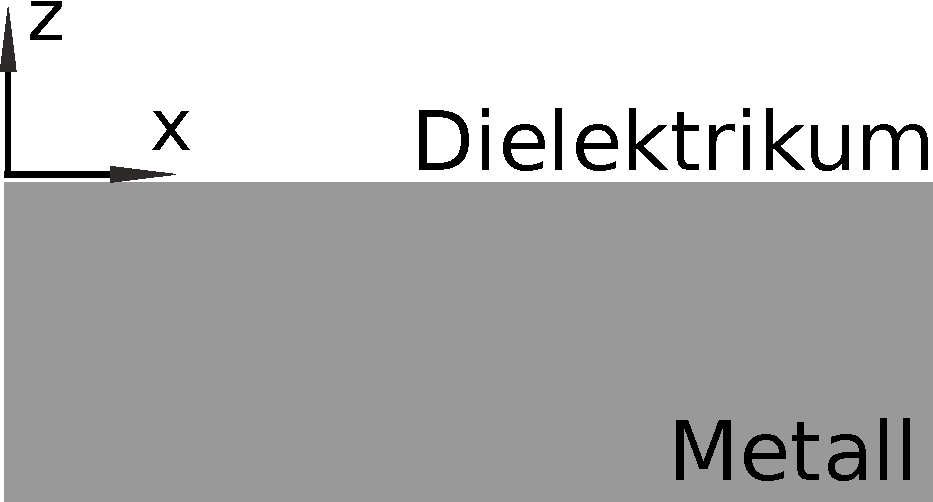
\includegraphics[scale=0.25]{images/leiter_und_nichtleiter.pdf}\\[-0.5\baselineskip]
            \hspace{1.5cm}}%        
    \end{column}        
    \end{columns}
\end{frame}

\begin{frame}{Oberflächenplasmon-Polariton}
    \begin{columns}
        \begin{column}{0.5\textwidth}
            \begin{itemize}
                \item <1-> Plasmonen lassen sich mit Licht anregen
                \bigskip
                \item <2-> Dispersionsrelation $k_\text{spp} = k_0 \sqrt{\frac{\epsilon_1 \,\epsilon_2}{\epsilon_1 + \epsilon_2}}$
                %\bigskip 
                \item <4-> Schnittpunkt: Energie- \& Impulserhaltung \rightarrow hier nicht \rightarrow keine Anregung
                \bigskip 
                \item <5-> Bedingung? \rightarrow Goldgitter auf Oberfläche nötig
                %\bigskip 
                \item <7-> $k_\text{SPP} = k \sin(\theta) \pm m \, G $ mit $m \in \mathbb{N}^+$ und $G = \frac{2 \, \pi}{a}$
               \bigskip 
                \item <8-> Prozess auch umgekehrt möglich. Plasmon kann als Licht auskoppeln.
            \end{itemize}
        \end{column}
        \begin{column}{0.5\textwidth}
            \centering
            \only <3->{
            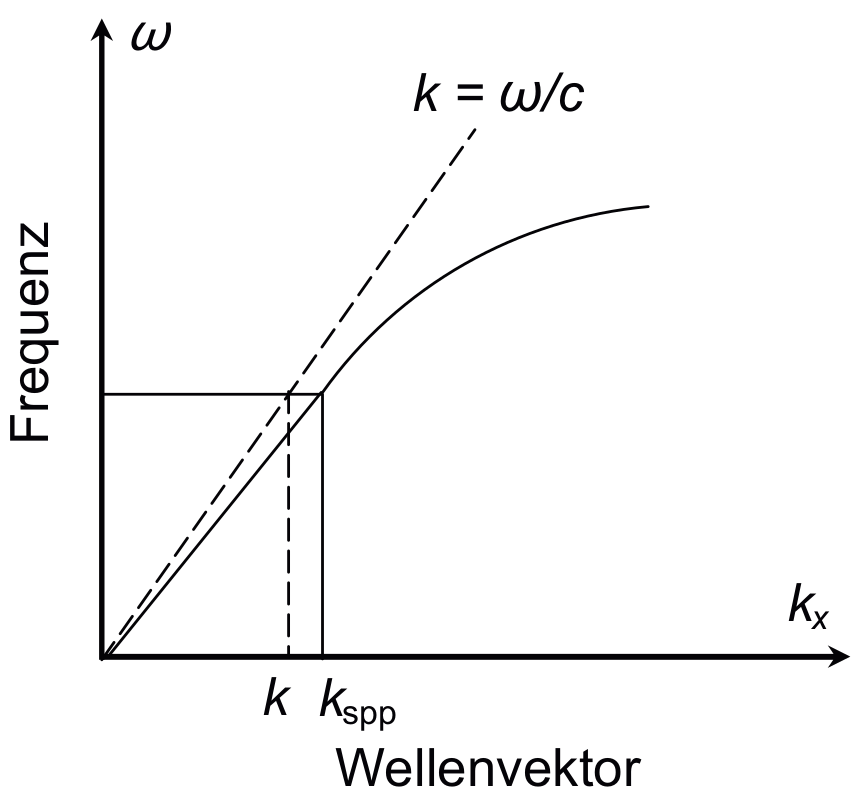
\includegraphics[width=3.5cm]{images/disp.png}\\ \hspace{1.5cm} {[{Stefan Maier, Plasmonics}]}
            }
            \only <6->{
            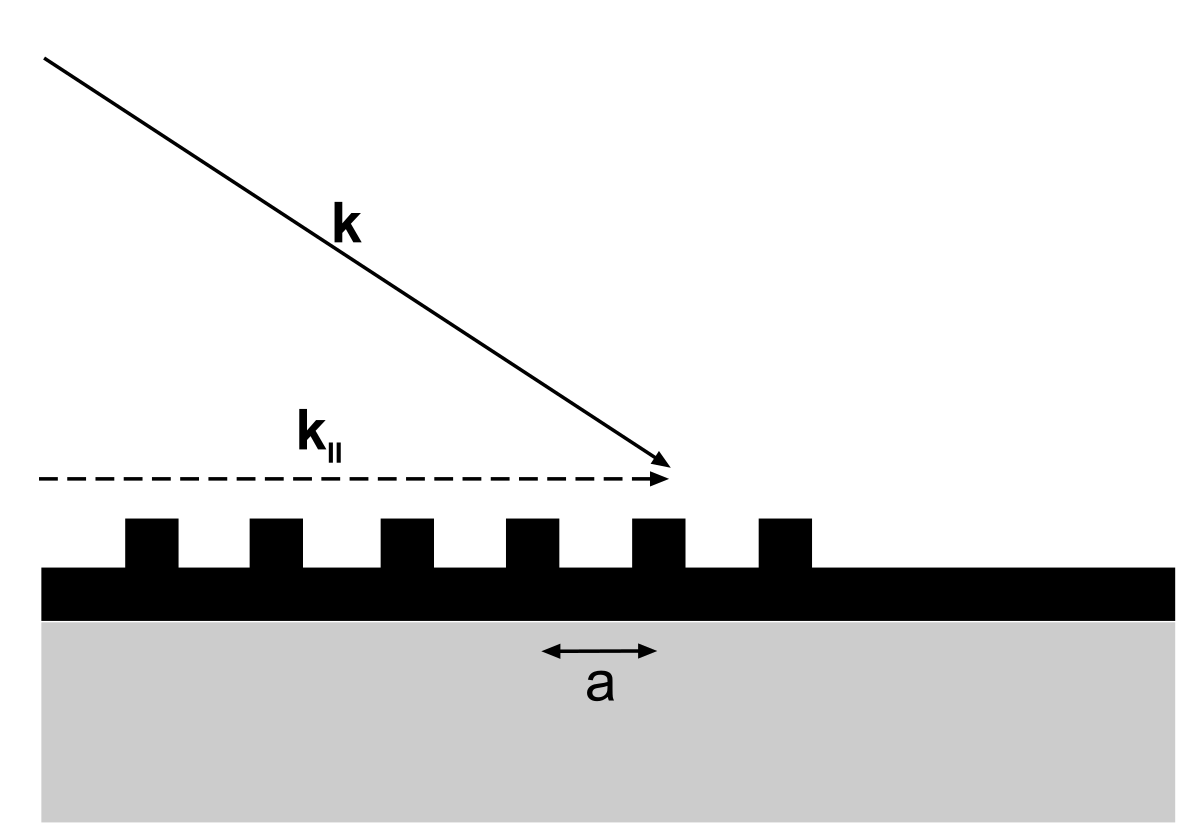
\includegraphics[width=3.5cm]{images/gitter.png}\\ \hspace{1.5cm} {[{Stefan Maier, Plasmonics}]}
            }
        \end{column}
    \end{columns}
\end{frame}

%\subsection{Große Zeemanaufspaltung}
\begin{frame}{Große Zeemanaufspaltung}
    \pause
    \begin{columns}
        \begin{column}{0.5\textwidth}
            \begin{itemize}
                \item <1-> Aufspaltung der Energieniveaus im Magnetfeld
                \item <3-> Magnetfeld in Voigt-Geometrie \rightarrow parallel zur Probenoberfläche 
                \item <4-> Aufspaltung von Leicht- (lh) und Schwerloch (hh) in jeweils 2 Niveaus
                \item <5-> blau, rot $\sigma \text{-Übergänge}$ \rightarrow beide zirkular Polarisiert in x-y-Ebene 
                \rightarrow Unterschied der Drehrichtung
                \item <6-> Schwerlochübergang am wahrscheinlichsten
                \item <7-> bei tiefen Temperaturen quasi nur Übergange in das Schwerlochband
            \end{itemize}
        \end{column}
        \begin{column}{0.5\textwidth}
            \centering
            \only <2->{
            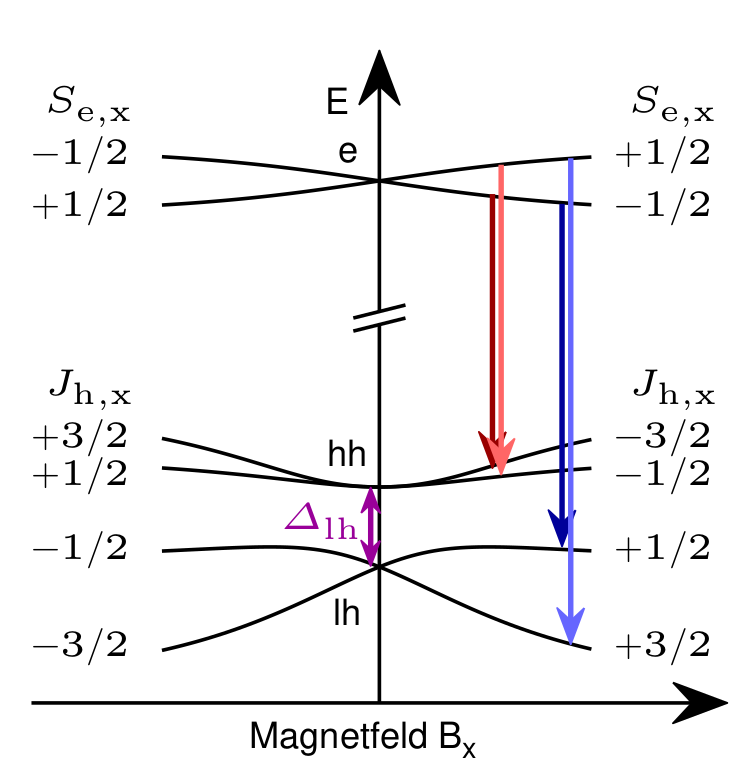
\includegraphics[scale=0.2]{images/zeeman.png}\\[-0.5\baselineskip]{[Felix Spitzer, Dissertation]}}
        \end{column}
    \end{columns}
\end{frame}

%\subsection{Magnetisch kontrollierte direktionale Lichtemission}
\begin{frame}{Magnetisch kontrollierte direktionale Lichtemission}
    \pause
    \begin{columns}
        \begin{column}{0.5\textwidth}
            \begin{itemize}
                \item <1-> Beschreibt wie mit Hilfe eines
                angelegten äußeren Magnetfelds die Lichtemission einer Probe gerichtet
                werden kann. 
                \bigskip   
                \item <3-> Laser erzeugt im Quantentopf der
                Probe Exzitonen als Quelle der Strahlung
                \bigskip   
                \item <4-> Emission der Exzitonen besitzen vorgegebene zirkulare Polarisation
                \bigskip
                \item <5->  Deckschicht: \SI{30}{\nano\meter}
                \item <5->  Quantentopf: \SI{10}{\nano\meter}
                \item <5->  Puffer: \SI{4,6}{\micro\meter}
            \end{itemize}
        \end{column}
        \begin{column}{0.5\textwidth}
            \centering
            \only <2->{
                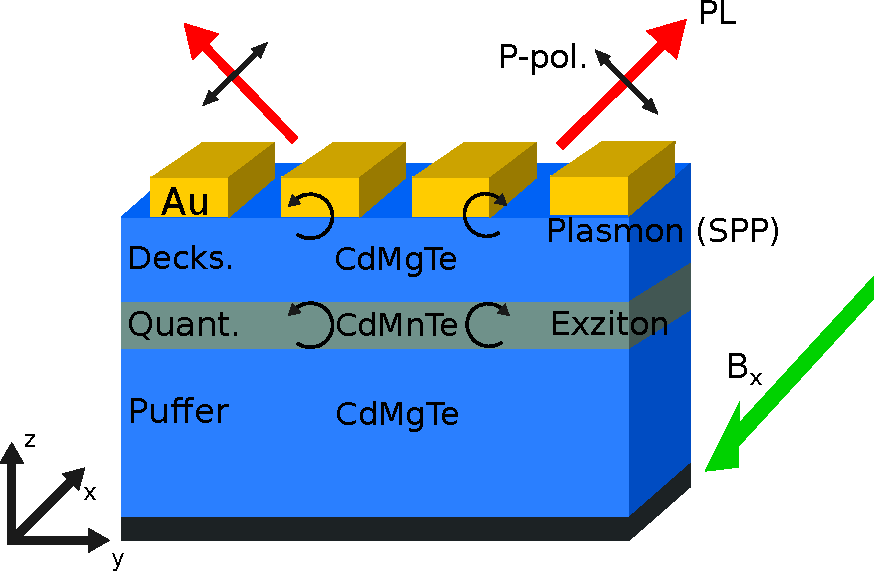
\includegraphics[scale=0.35]{images/Probe_komplett.pdf}\\[-0.5\baselineskip]
                }
        \end{column}
    \end{columns}
\end{frame}

\begin{frame}{Magnetisch kontrollierte direktionale Lichtemission}
    \begin{columns}
        \begin{column}{0.5\textwidth}
            \begin{itemize}
                \item <1-> für $B_{x} = 0$ zirkulare Emission der Exzitonen nur in der x-y-Ebene
                \item <3-> für $B_{x} \neq 0$ zirkulare Emission der Exzitonen erscheinen in der y-z-Ebene
                elliptisch polarisiert 
                \item <4-> Grad der zirkularen Polarisation
                \begin{equation*}
                    P_c \approx \frac{2}{3} \frac{\Delta_\text{h,F}(T)}{\Delta_\text{lh}} \propto B
                    \label{eq:pc}
                \end{equation*}
                \item <5-> Exzitonen können mit Plasmonen mit gleicher Polarisation koppeln 
                \item <6-> Plasmonen emittieren als Licht \rightarrow direktionale Lichtemission
                \item <7-> Steuerung durch Magnetfeld möglich \rightarrow transversale magnetische Führung der Lichtemission (TMRLE)
            \end{itemize}
        \end{column}
        \begin{column}{0.5\textwidth}
            \centering
            \only <2->{
                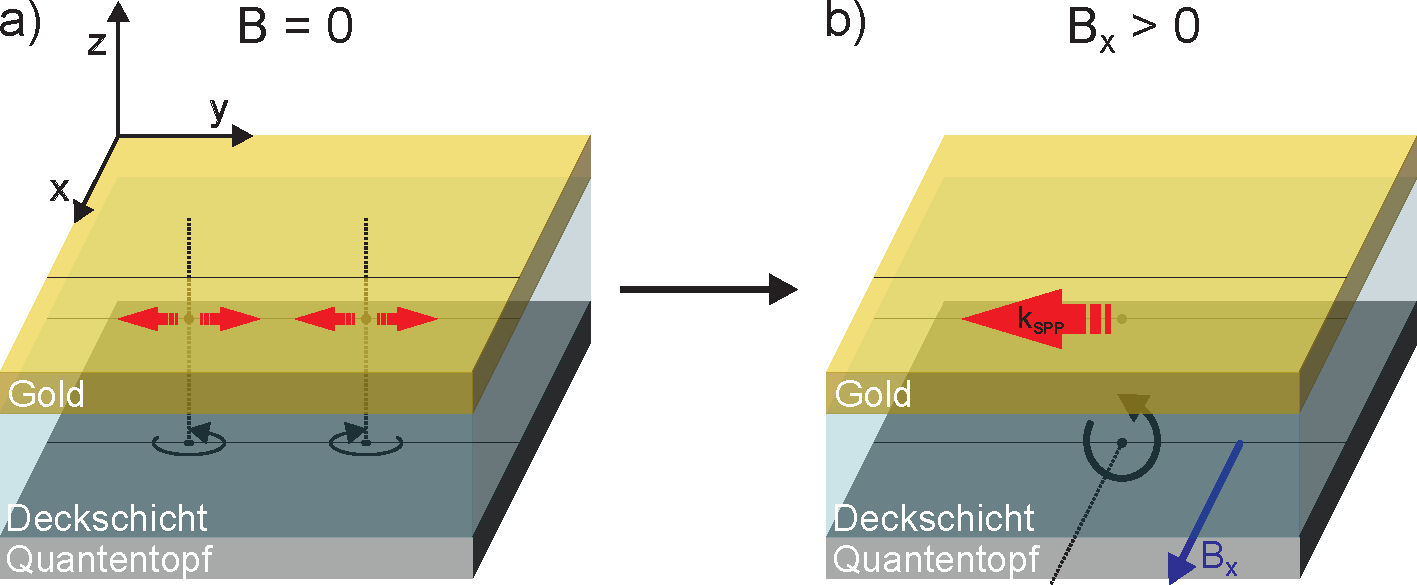
\includegraphics[scale=0.25]{images/exziton.pdf}\\[-0.5\baselineskip]{[Lars Klompmaker, Masterarbeit]}
             }
        \end{column}
    \end{columns}
\end{frame}

%\subsection{Temperaturabhängigkeit der magnetisch kontrollierten direktionale Lichtemission}
\begin{frame}{Temperaturabhängigkeit der magnetisch kontrollierte direktionale Lichtemission}
    \begin{columns}
        \begin{column}{0.5\textwidth}
            \begin{itemize}
                \item <1-> $\Delta_\text{h,F}(T)$ ist temperaturabhängig  
                \rightarrow $\Delta_\text{h,F}(T) = xN_0\beta \bigl< S^\text{Mn}_{z} \bigr>$
                \item <2-> $\bigl< S^\text{Mn}_{z} \bigr>$ ist die mittlere thermische Spinausrichtung der Mn-Ionen entlang des angelegten
                Magnetfelds 
                \item <3->
                \begin{align*}
                    \label{eq:S}
                    \bigl< S^\text{Mn}_{z} \bigr> &= S_\text{eff} B_\text{$\frac{5}{2}$} \left(\frac{5}{2}\frac{g_\text{Mn} \mu_\text{B} B }{T_\text{eff} k_\text{B}} \right)\text{.}
                \end{align*}
                \bigskip
                \item <4-> anschaulich \rightarrow mit steigender Temperatur wird die Spinausrichtung schlechter 
                \item <5-> $P_\text{c}$ sinkt \rightarrow Verlust der Direktionaltät
                %\item <->
            \end{itemize}
        \end{column}
        \begin{column}{0.5\textwidth}
            \centering
            \only <1->{
                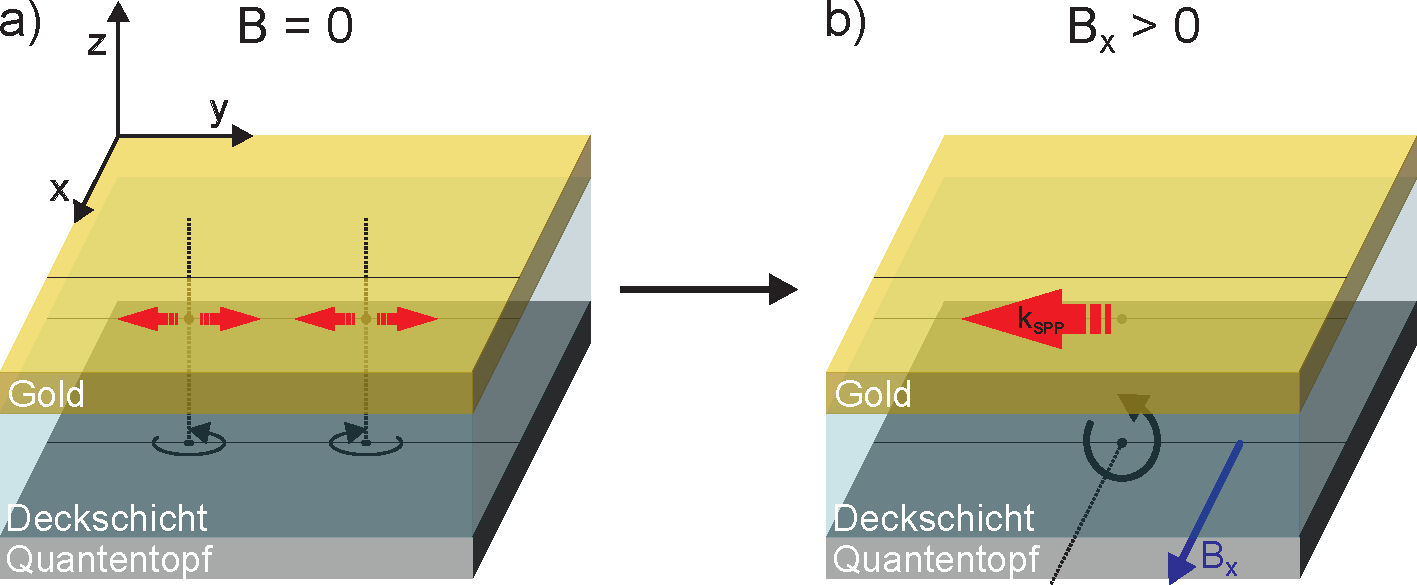
\includegraphics[scale=0.25]{images/exziton.pdf}\\[-0.5\baselineskip]{[Lars Klompmaker, Masterarbeit]}                
            }
            %\only <6->{
            %    \bigskip 
            %    \begin{align*}
            %        P_c \approx \frac{2}{3} \frac{\Delta_\text{h,F}(T)}{\Delta_\text{lh}} \propto B
            %    \end{align*}
            %}
        \end{column}
    \end{columns}
\end{frame}